%%%%%%%%%%%%%%%%%%%%%%%%%%%%%%%%%%%%%%%%%%%%%%%%%%%%%%%%%%%%%%%%%%%%%%%%%%%%%%%%
%2345678901234567890123456789012345678901234567890123456789012345678901234567890
%        1         2         3         4         5         6         7         8

\documentclass[letterpaper, 10 pt, conference]{ieeeconf}  % Comment this line out if you need a4paper

%\documentclass[a4paper, 10pt, conference]{ieeeconf}      % Use this line for a4 paper

\IEEEoverridecommandlockouts                              % This command is only needed if 
                                                          % you want to use the \thanks command

\overrideIEEEmargins                                      % Needed to meet printer requirements.
\usepackage{graphicx}
\usepackage{amsmath}

%In case you encounter the following error:
%Error 1010 The PDF file may be corrupt (unable to open PDF file) OR
%Error 1000 An error occurred while parsing a contents stream. Unable to analyze the PDF file.
%This is a known problem with pdfLaTeX conversion filter. The file cannot be opened with acrobat reader
%Please use one of the alternatives below to circumvent this error by uncommenting one or the other
%\pdfobjcompresslevel=0
%\pdfminorversion=4

% See the \addtolength command later in the file to balance the column lengths
% on the last page of the document

% The following packages can be found on http:\\www.ctan.org
%\usepackage{graphics} % for pdf, bitmapped graphics files
%\usepackage{epsfig} % for postscript graphics files
%\usepackage{mathptmx} % assumes new font selection scheme installed
%\usepackage{times} % assumes new font selection scheme installed
%\usepackage{amsmath} % assumes amsmath package installed
%\usepackage{amssymb}  % assumes amsmath package installed

\title{\LARGE \bf
Sensor Synergy of Lidar and Vision-Based Detection for Obstacle Mapping and Depth Estimation in the KITTI Dataset
}


\author{Gaurav Surtani}



\begin{document}



\maketitle
\thispagestyle{empty}
\pagestyle{empty}


%%%%%%%%%%%%%%%%%%%%%%%%%%%%%%%%%%%%%%%%%%%%%%%%%%%%%%%%%%%%%%%%%%%%%%%%%%%%%%%%
\begin{abstract}

In the evolving field of autonomous vehicle development, there's a common reliance on single-sensor systems for navigational decision-making. This project proposes augmenting Lidar with an additional sensor to enhance safety and decision-making through sensor fusion. The study will investigate the sequential integration of Lidar with an auxiliary sensor to evaluate effectiveness in improving obstacle detection. By examining different sensor fusion methodologies, the project aims to determine if a multi-sensor approach can quicken and refine the environmental scanning process. This simulation-based study intends to narrow the gap between theoretical sensor fusion models and practical, scalable real-world autonomous driving applications.

\end{abstract}

\begin{keywords}
Autonomous Vehicles, Sensor Fusion, Lidar, Obstacle Detection, Multi-Sensor Integration, KITTI Raw Data, Simulation-Based Study, Rigid Body Transformations
\end{keywords}


%%%%%%%%%%%%%%%%%%%%%%%%%%%%%%%%%%%%%%%%%%%%%%%%%%%%%%%%%%%%%%%%%%%%%%%%%%%%%%%%
\section{INTRODUCTION}

\subsection{Sensor Fusion}
Autonomous cars employ multiple sensor types to enhance detection reliability and precision. This diversity and redundancy in sensors ensure more accurate readings by cross-verifying data. 

Each sensor used for detecting objects has its unique strengths and weaknesses. By combining these sensors through sensor fusion, the detection becomes more precise and robust. For example, cameras are excellent at capturing detailed texture and color information, something that LiDAR typically does not provide. Conversely, LiDAR excels in conditions of low visibility, like nighttime or during light fog or rain. \cite{NVIDIA}

\begin{figure}[htbp]
  \centering
  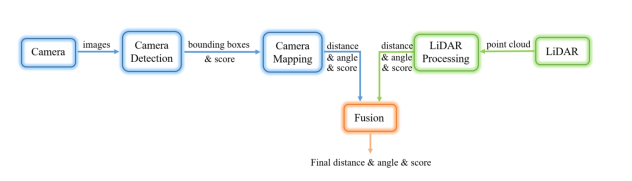
\includegraphics[width=\linewidth]{fusion.png}
  \caption{Sensor Fusion Apporach}
  \label{Sensor Fusion}
\end{figure}	

\subsection{LiDAR}   
In a LiDAR system, thousands of laser pulses are emitted every second to detect objects around the vehicle. These pulses reflect off objects and return to the sensor, creating a 3-D point cloud. An onboard computer then rapidly translates these reflections into an animated 3-D representation. While LiDAR excels in measuring distances, it falls short in providing a dense, rich representation of the environment, a task where cameras outperform. Cameras, however, struggle with accurately measuring distances. Understanding LiDAR data can be challenging, as it does not readily identify the type of detected objects. In contrast, camera imagery offers clarity in differentiating between objects like cars and signposts. This complementary functionality of LiDAR and cameras enhances the overall perception capability of autonomous vehicles.

\subsection{Why Fuse Camera and LiDAR}   
The choice to use both Cameras and LiDAR in autonomous vehicles is a strategic one, balancing their respective strengths and weaknesses. LiDAR is great for creating high-resolution 3D maps and measuring distances accurately, and it works well in different lighting and some harsh weather conditions. It can even see through obstacles like foliage. But, it's expensive, bulky, and its data is complex. Plus, it doesn't handle heavy rain or snow well.

On the other hand, Cameras are more budget-friendly, compact, and the data they produce is easier to process. They capture the world in color, which LiDAR can't do. However, they rely heavily on good lighting, only provide 2D images, and struggle with distance measurements. Weather conditions can also hamper their effectiveness.

By combining these two technologies, autonomous vehicles can get a fuller, more accurate picture of their surroundings, making up for the limitations of each system.

\begin{figure}[htbp]
  \centering
  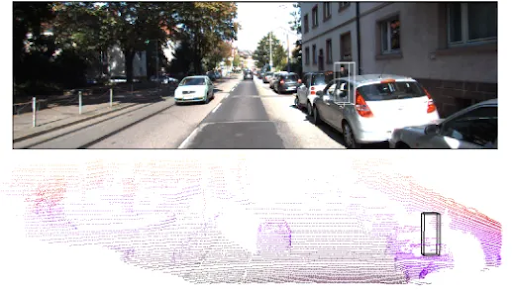
\includegraphics[width=\linewidth]{whylidarcamera.png}
  \caption{Results from the base setup.}
  \label{Why Lidar and Camera}
\end{figure}

\subsection{KITTI Vehicle}
The KITTI dataset, developed by the Karlsruhe Institute of Technology and Toyota Technological Institute at Chicago, is a benchmark suite for autonomous driving tasks. It includes a range of datasets captured in urban environments, focusing on several tasks crucial for autonomous driving, such as stereo, optical flow, visual odometry, 3D object detection, and 3D tracking. This dataset is particularly notable for its real-world relevance, featuring various urban scenarios and conditions. It has been widely used in the research community for testing and developing advanced driver-assistance systems and autonomous driving technologies. \cite{KITTI}

\begin{figure}[htbp]
  \centering
  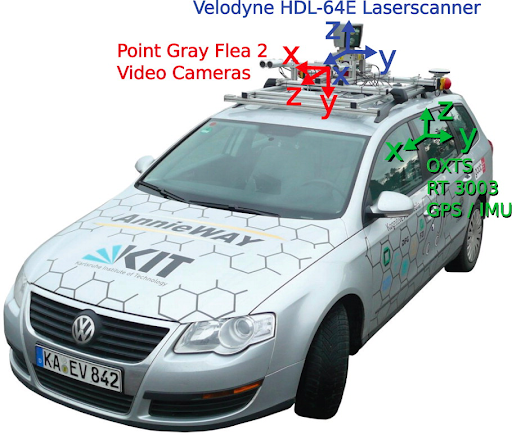
\includegraphics[width=\linewidth]{KITTI_car.png}
  \caption{KITTI Car Representation}
  \label{KITTI Ego Vehile}
\end{figure}

\subsection{KITTI Dataset}

From the KITTI website\cite{KITTIWebsite}, we are going to use their raw data to do the sensor fusion between the Camera and LiDAR.
A little brief information on the different types of data provided by KITTI and what do they signify:

\begin{itemize}
  \item Stereo Sequences: Both raw (unsynced+unrectified) and processed (synced+rectified) in grayscale and color, with 0.5 Megapixels resolution, stored in PNG format.
  \item 3D Velodyne Point Clouds: Capturing 100k points per frame, stored as a binary float matrix.
  \item 3D GPS/IMU Data: Providing location, speed, acceleration, and meta-information, stored as text files.
  \item Calibration Data: Including camera and sensor calibration details, stored as text files.
  \item 3D Object Tracklet Labels: For objects like cars, pedestrians, stored in XML format.
\end{itemize}

In the KITTI dataset, the terms "unsynced" and "synced" are pivotal in understanding the temporal characteristics of the sensor data. "Unsynced" data refers to instances where the output from various sensors is not temporally aligned, resulting in disparate data streams that do not correspond to identical time frames. Conversely, "synced" data signifies that the sensor outputs are meticulously aligned in time, ensuring that each sensor's data corresponds precisely to the same temporal moment. This synchronization is crucial for tasks that necessitate the integrated analysis of multiple sensor modalities, as it guarantees consistency and accuracy in the temporal domain.


\begin{figure}[htbp]
  \centering
  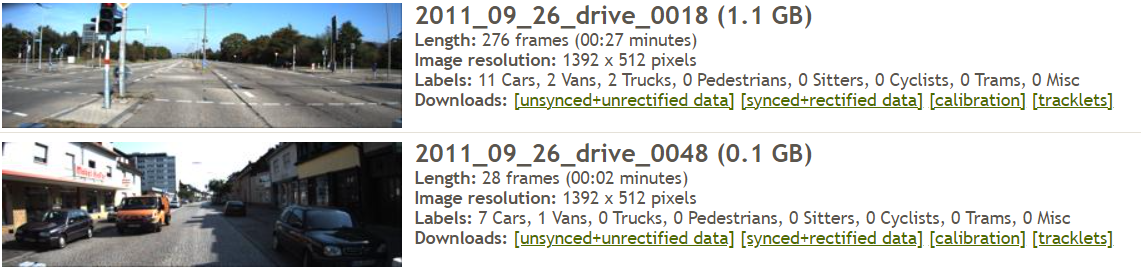
\includegraphics[width=\linewidth]{raw_data_KITTI.png}
  \caption{KITTI Raw Data Files}
  \label{KITTI Raw Data}
\end{figure}


\section{Methodology}

\subsection{Sensor Setup}

We'll be using the KITTI vehicle which has 4 cameras; 2 grayscale and 2 RGB, the velodyne HDL64-E LiDAR.

From the original paper \cite{KITTI} , we have the following sensor setup information about the KITTI vehicle illustrated in Fig. 3:
\begin{itemize}
  \item 2 $\times$ PointGray Flea2 grayscale cameras (FL2-14S3M-C), 1.4 Megapixels, 1/2'' Sony ICX267 CCD, global shutter.
  \item 2 $\times$ PointGray Flea2 color cameras (FL2-14S3C-C), 1.4 Megapixels, 1/2'' Sony ICX267 CCD, global shutter.
  \item 4 $\times$ Edmund Optics lenses, 4mm, opening angle $\approx 90^\circ$, vertical opening angle of region of interest (ROI) $\approx 35^\circ$.
  \item 1 $\times$ Velodyne HDL-64E rotating 3D laser scanner, 10 Hz, 64 beams, 0.09 degree angular resolution, 2 cm distance accuracy, collecting $\approx 1.3$ million points/second, field of view: 360$^\circ$ horizontal, 26.8$^\circ$ vertical, range: 120 m.
  \item 1 $\times$ OXTS RT3003 inertial and GPS navigation system, 6 axis, 100 Hz, L1/L2 RTK, resolution: 0.02m / 0.1$^\circ$.
\end{itemize}

Since the update rate differs between various sensors we'll be using the synced data provided in raw data set of KITTI, we shall be syncing the 10Hz LidAR along with 15fps Camera. There may be neglible error of 5ms for some images and LiDAR data fused according to the base paper.

\begin{figure}[htbp]
  \centering
  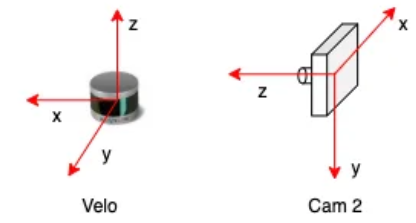
\includegraphics[width=\linewidth]{sensor_directions.png}
  \caption{Sensor Direction Layout}
  \label{Sensor Direction Layout}
\end{figure}

From Fig 5. , we understand the orientation and data provided by Camera and LiDAR. For the camera, the direction the vehicle is moving towards is z, along later we see that this value will depict the depth of a particular object detected by the LiDAR. 

On the other hand, LiDAR has different orientation, the vehicle accelerates in the x direction, y is perpendicular to that. z is the height that the point is in the Point Cloud Bin File above the ground.

Sensor Fusion involves integrating data from multiple sensors, a process complicated by their disparate locations and orientations. To effectively merge these data streams, it's essential to apply appropriate coordinate transformations. This necessitates precise knowledge of each sensor's position on the ego vehicle. Fortunately, this information is readily available in the form of a diagram (Fig. 6) provided in the KITTI paper \cite{KITTI}.

\begin{figure}[htbp]
  \centering
  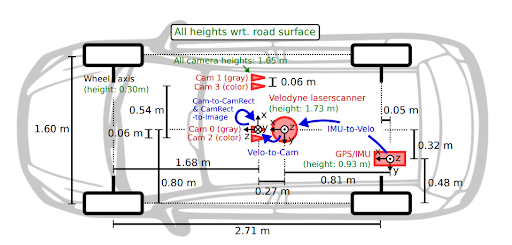
\includegraphics[width=\linewidth]{KITTI_Layout.png}
  \caption{KITTI Sensors Layout}
  \label{KITTI Sensors Layout}
\end{figure}

From Fig (7), we can clearly explore the data provided to us by the sycned KITTI raw data.
We see the data from the four cameras; 1,2,3 and 4. Each camera has an image for four cameras, all are different positions of the ego vehicle in KITTI.
Each Frame from the camera corresponds to one image from all the cameras. 

The Velodyne points contains .bin file which are used to depict the Point Cloud Library of each frame corresponding to every image in the above directories.

The calibration files are the crux of this project, we will be focusing convert the LiDAR data to data understandable by a reference camera.
There are multiple ways to do this; we can use the LiDAR data and convert it Camera 0 data or we can to do Camera 2 data.


\begin{figure}[htbp]
  \centering
  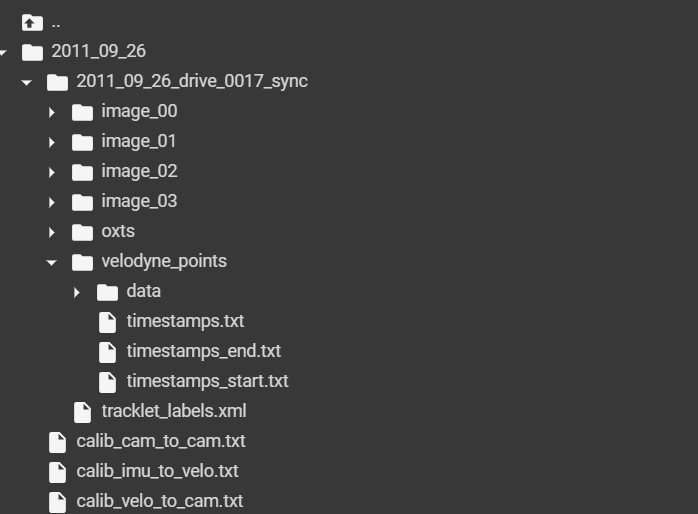
\includegraphics[width=\linewidth]{folder-struct.png}
  \caption{File Structure Layout}
  \label{File Structure Layout}
\end{figure}


\subsection{Sensor Calibration}

The Rigid Body Transformation will allow us to convert from one sensor's coordinate system to another. In equation \ref{eq:rigid_body_transformation}, the rotation \( \mathbf{R} \) is a \( 3 \times 3 \) matrix and the translation \( \mathbf{t} \) is a \( 3 \times 1 \) vector. We can concatenate these together and advantageously express this transformation in matrix form as:

\begin{equation}
\mathbf{T}(\mathbf{v}) = \mathbf{Rv} + \mathbf{t}
\label{eq:rigid_body_transformation}
\end{equation}

\textit{Equation 1. Rigid Body Transformation on \( \mathbf{v} \) with rotation \( \mathbf{R} \) and translation \( \mathbf{t} \).}


where we can express the transformation matrix \( \mathbf{T} \) as:

\begin{equation}
\mathbf{T} = \begin{bmatrix}
r_{11} & r_{12} & r_{13} & t_{14} \\
r_{21} & r_{22} & r_{23} & t_{24} \\
r_{31} & r_{32} & r_{33} & t_{34} \\
\end{bmatrix}
\label{eq:transformation_matrix}
\end{equation}

\textit{Equation 2. Rigid Body Transformation Matrix.}
	


Where the \( r \)'s correspond to the \( 3 \times 3 \) rotation matrix and the \( t \)'s correspond to the \( 3 \times 1 \) translation vector. When working with the KITTI data set, we will need to use many transformation matrices, thankfully we can find them all in the KITTI calibration data, see the KITTI README for more information. (The calibration files typically come with each downloadable data set from KITTI).


In our approach, we employ homogeneous transformations to map data from the LiDAR system to the camera's coordinate system, ensuring compatibility and coherence in data interpretation between these sensors.

\begin{figure}[htbp]
  \centering
  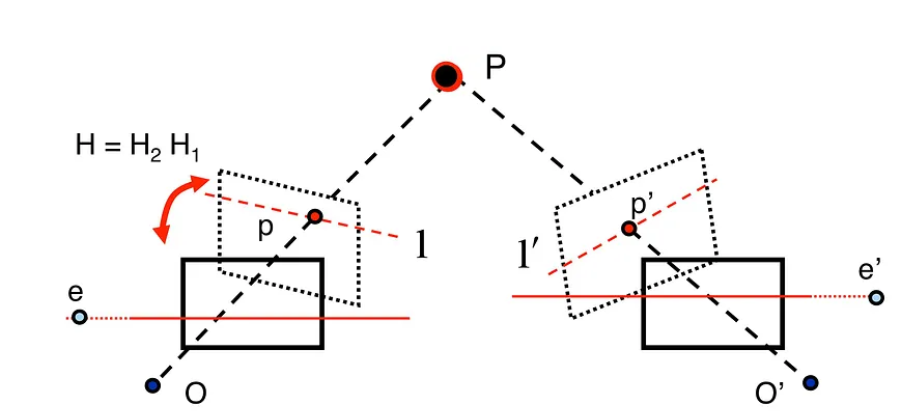
\includegraphics[width=\linewidth]{rigidbodytran.png}
  \caption{P(i) Rect}
  \label{P(i) Rect}
\end{figure}

The calibration procedure is anchored around camera 0 (cam0), designated as the reference sensor. This setup is crucial as it dictates the alignment of the laser scanner in accordance with the reference camera's coordinate system. Moreover, the calibration process incorporates the rectification matrix, denoted as \textit{R\_ref2rect}, which is instrumental in addressing and correcting planar misalignments between the cameras.

The rectification process encompasses several vital components:
\begin{itemize}
  \item \textit{P\_rect[i]}: Denotes the projective transformation from the rectified frame of the reference camera to camera \textit{i}. Here, \textit{bx[i]} represents the baseline in relation to the reference camera 0.
\begin{figure}[htbp]
  \centering
  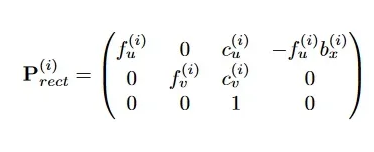
\includegraphics[width=\linewidth]{PiRect.png}
  \caption{Rigid Body Transformation}
  \label{Rigid Body Transformation}
\end{figure}
  \item \textit{R0\_rect}: A rotation matrix used to rectify points within the reference camera frame.
  \item \textit{Tr\_velo\_to\_cam}: Refers to the Euclidean transformation from the LiDAR system to the reference camera cam0.
\end{itemize}
These parameters are integral to achieving precise data alignment and transformation across the different sensors in the dataset.

To summarize, Rigid Body Transformation is used to scale the data from the images negate the error from the position of the camera, translate and rotate the image so as to get an image from the reference camera. This can be the converted from to Homogenous equation adding a fourth row with the last element as 1.


\subsection{Transform LiDAR to Camera}

To map a LiDAR point cloud to the camera image space, we perform a series of transformations on each point. The focus is on transforming points to Camera 2 (the left color image), the derived equations are adaptable for translating LiDAR points to any camera. We employ homogeneous coordinates for these transformations. To express a transformation matrix in homogeneous form, we append a row at the bottom, placing zeros beneath the rotation and a one beneath the translation as seen below in equation (3).

\begin{equation}
\mathbf{T} = \begin{bmatrix}
r_{11} & r_{12} & r_{13} & t_{14} \\
r_{21} & r_{22} & r_{23} & t_{24} \\
r_{31} & r_{32} & r_{33} & t_{34} \\
0 & 0 & 0 & 1
\end{bmatrix}
\label{Equation 3. Homogeneous Rigid Body Transformation.}
\end{equation}

A LiDAR point is initially a \(3 \times 1\) vector, which we convert to homogeneous coordinates by appending a one in the fourth dimension, resulting in a \(4 \times 1\) vector. Homogeneous coordinates simplify the representation, enabling us to express all transformations in matrix form. The summary of the transformation process includes 'velo' for LiDAR, 'ref\#' for the physical camera locations, 'rect\#' for the rectified camera rotations, and 'cam\#' for the 2D camera locations.

\begin{equation}
\tilde{\mathbf{y}} = \mathbf{P}_{\text{cam2}}^{\text{rect2}} \mathbf{R}_{\text{rect2}}^{\text{ref2}} \mathbf{R}_{\text{ref2}}^{\text{ref0}} \mathbf{R}_{\text{ref0}}^{\text{velo}} \tilde{\mathbf{x}}, \quad \text{where} \quad \tilde{\mathbf{x}} = [x, y, z, 1]^T
\label{eq:lidar_to_camera_transformation}
\end{equation}


The subscripts in each transformation matrix in Equation 4 denote the source coordinate system, while the superscripts indicate the target system.

To revert from homogeneous coordinates:

\begin{equation}
\mathbf{y} = \left( \frac{\tilde{u}}{\tilde{z}}, \frac{\tilde{v}}{\tilde{z}}, \tilde{z} \right)
\label{eq:convert_from_homogeneous}
\end{equation}


We initiate the sequence of transformations by converting points from the LiDAR frame to the camera 0 frame of reference. The camera frame of reference is a 3D point in the world relative to the location of camera 0 on the ego vehicle.

The subsequent transformation is a rigid body transformation from Camera 0 to Camera 2 (or any desired camera). Then, we apply the rectifying transformation, which is a rotation necessary for working with stereo images that share the same y-axis, ensuring that objects on both images align vertically. This process is known as rectification. \cite{CoordinateTransforms}

Lastly, we execute the camera projection transformation, which maps the location of a 3D point into 2D image space, denoted as \( (u, v) \) or \( (u, v, z) \) when depth information is available. Note that the rectifying transformation is prerequisite for this projection to be valid.

\begin{equation}
\mathbf{T}_{\text{cam2}}^{\text{velo}} = \mathbf{P}_{\text{cam2}}^{\text{rect2}} \mathbf{R}_{\text{rect2}}^{\text{ref2}} \mathbf{R}_{\text{ref2}}^{\text{ref0}} \mathbf{T}_{\text{ref0}}^{\text{velo}}
\label{eq:transformation_matrix_lidar_camera}
\end{equation}

\begin{itemize}
  \item $\mathbf{T}_{\text{ref0}}^{\text{velo}}$ - LiDAR to Camera Reference — transforms a 3D point relative to the LiDAR to a 3D point relative to the Camera
  \item $\mathbf{R}_{\text{ref2}}^{\text{ref0}}$ - Rigid Body Transformation from Camera 0 to Camera 2
  \item $\mathbf{R}_{\text{rect2}}^{\text{ref2}}$ - Camera 2 to Rectified Camera 2 reference
  \item $\mathbf{P}_{\text{cam2}}^{\text{rect2}}$ - Rectified Camera 2 to 2D Camera 2 (\(u, v, z\)) coordinate space
  \item $\mathbf{T}_{\text{cam2}}^{\text{velo}}$ - 3D LiDAR space to 2D Camera 2 (\(u, v, z\)) coordinate space.
\end{itemize}
Note: We still denote \((u, v, z)\) as 2D space even though we have \(z\) since we are referring to the 2D camera image space with real world depth relative to the camera.


\subsection{Projection from Camera to LiDAR Coordinates}

Annotations of 3D bounding boxes are typically provided in the camera coordinate frame. To convert these box vertices from the camera frame to the LiDAR frame, one must apply the inverse of the rigid transformation used for the camera to LiDAR projection. This process involves computing the inverse matrices and applying them in reverse order.

\begin{figure}[htbp]
  \centering
  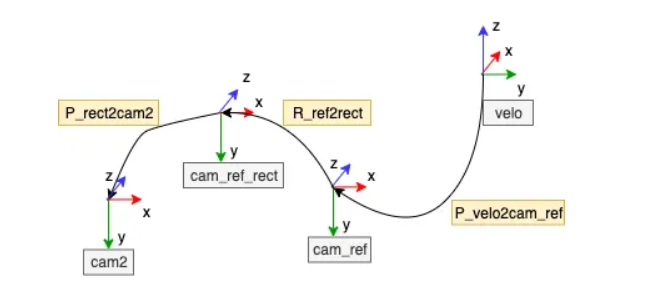
\includegraphics[width=\linewidth]{lidarconversiontocamera.png}
  \caption{Lidar to Camera Conversion}
  \label{ Lidar to Camera Conversion}
\end{figure}

Firstly, we compute the inverse of the rectification transformation matrix:
\begin{equation}
\mathbf{R}_{\text{rect2}}^{\text{ref2}^{-1}} = \text{np.linalg.inv}(\mathbf{R}_{\text{ref2}}^{\text{rect2}})
\end{equation}

Then, we calculate the inverse of the projection matrix from the camera to the LiDAR frame:
\begin{equation}
\mathbf{P}_{\text{cam2}}^{\text{velo}^{-1}} = \text{np.linalg.inv}(\mathbf{T}_{\text{velo}}^{\text{cam2}})
\end{equation}

The overall projection matrix that transforms points from the camera frame to the LiDAR frame is given by the product of the inverses:
\begin{equation}
\mathbf{proj\_mat} = \mathbf{R}_{\text{rect2}}^{\text{ref2}} @ \mathbf{P}_{\text{cam2}}^{\text{velo}}
\end{equation}

Applying this projection matrix to the vertices of the 3D bounding boxes will transform them into the LiDAR coordinate frame.

\section{Object Detection}

For object detection, I will be using YoloV5 library. Since the primary focus of this paper was not object detection or image classification, we used Yolo pretrained model for detecting cars.
we use YoLo to give us the 2D bounding boxes provided from the image. Each array row delineates a detected bounding box and associated metrics:
\begin{enumerate}
    \item \textbf{Bounding Box Coordinates:}
    \begin{itemize}
        \item \(x_{\min}\): The x-coordinate of the top-left corner.
        \item \(y_{\min}\): The y-coordinate of the top-left corner.
        \item \(x_{\max}\): The x-coordinate of the bottom-right corner.
        \item \(y_{\max}\): The y-coordinate of the bottom-right corner.
    \end{itemize}
    
    \item \textbf{Confidence Score:}
    The fifth value denotes the confidence score, reflecting the detection's accuracy.
    
    \item \textbf{Class ID:}
    The sixth value represents the class ID, linking to the type of the detected object, defined as per the YOLO model's dataset.
    
    \item \textbf{Center Coordinates and Object Size:}
    The seventh and eighth values indicate the bounding box's center coordinates \((x_{\text{center}}, y_{\text{center}})\), with the ninth value likely representing a dimension of the object's size.
\end{enumerate}

But then again, to summarize everything up, this implementation just uses Yolo just for detecting the bounding boxes for all the object detected. [Refer to Figure 11 below]

\begin{figure}[htbp]
  \centering
  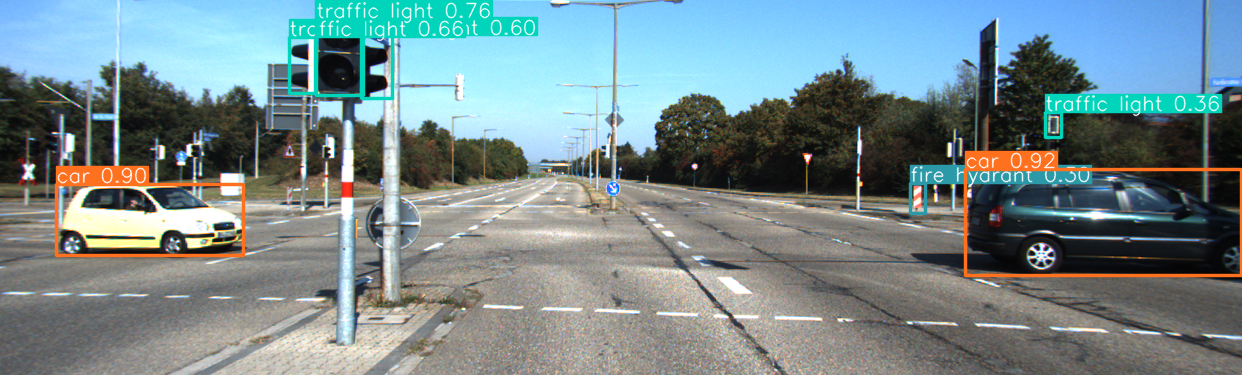
\includegraphics[width=\linewidth]{YoloDetectedImage.png}
  \caption{YoLo detected Image}
  \label{YoLo detected Image}
\end{figure}

The LiDAR uses these points are reference to detect the center of the bounding box detected by Yolo.
If we didn't use this, since LiDAR data reads a lot of data, it tends to pick up a lot of noise with respect to all the points surronding the center of the bounding box.
For ease of implementation, we use the data of Yolo detected center co-ordinates as the reference point that LiDAR needs to calculate the `z` or the depth of the object.



\section{Results}

Here in below; we shall see the different steps of how we are reaching our data fusion.
\begin{figure}[htbp]
  \centering
  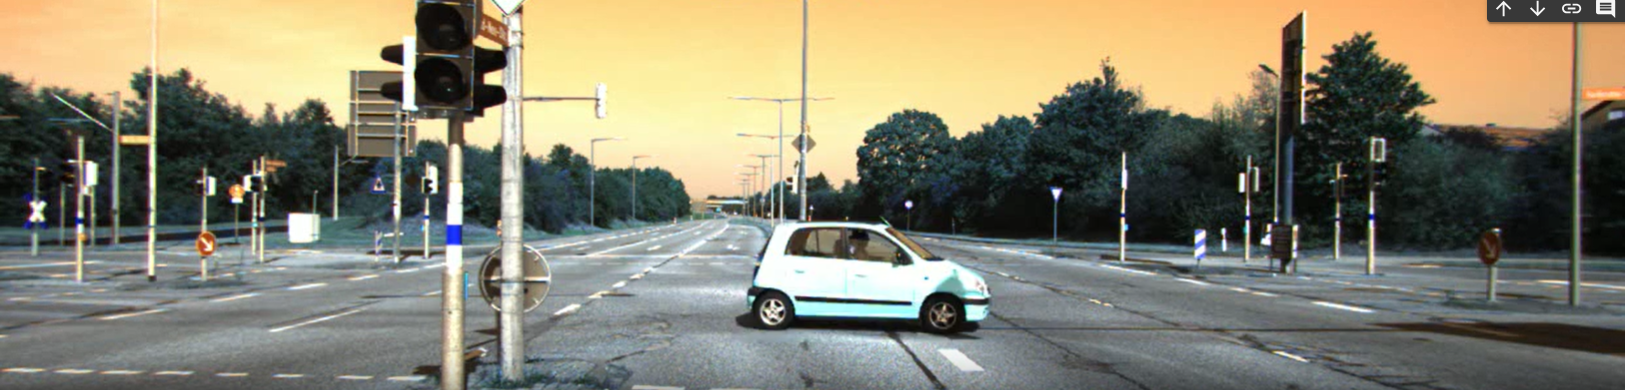
\includegraphics[width=\linewidth]{OnlyCamera.png}
  \caption{Only Camera Data}
  \label{Only Camera Data}
\end{figure}

The image[Fig. 12] above consists of camera data, that has been transformed using the equations in the sensor setup using Rigid Transformations.

\begin{figure}[htbp]
  \centering
  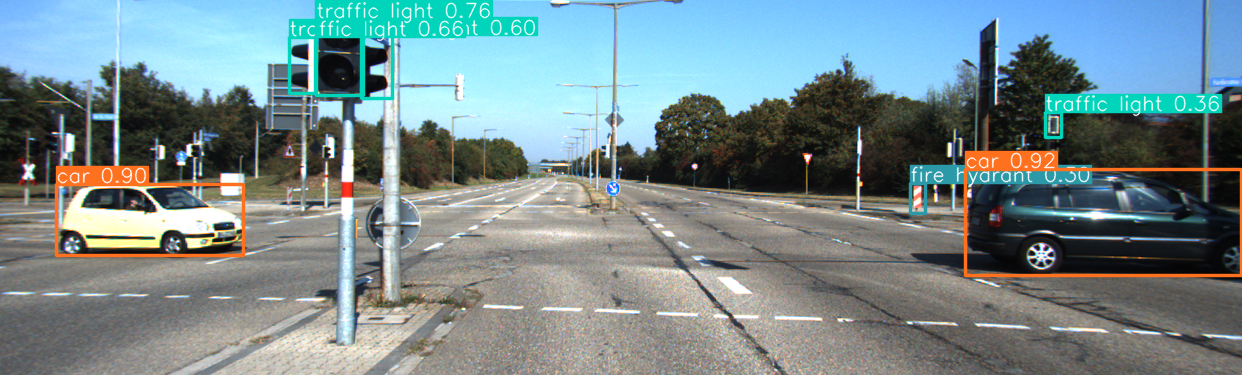
\includegraphics[width=\linewidth]{YoloDetectedImage.png}
  \caption{YoLo detected Image}
  \label{YoLo detected Image}
\end{figure}

The image[Fig 13] is then fed to the pre-trained Yolo model to detect vehicles and calculate the bounding boxes and find the center x and y of the box for the LiDAR to use to find the distance to that object.

\begin{figure}[htbp]
  \centering
  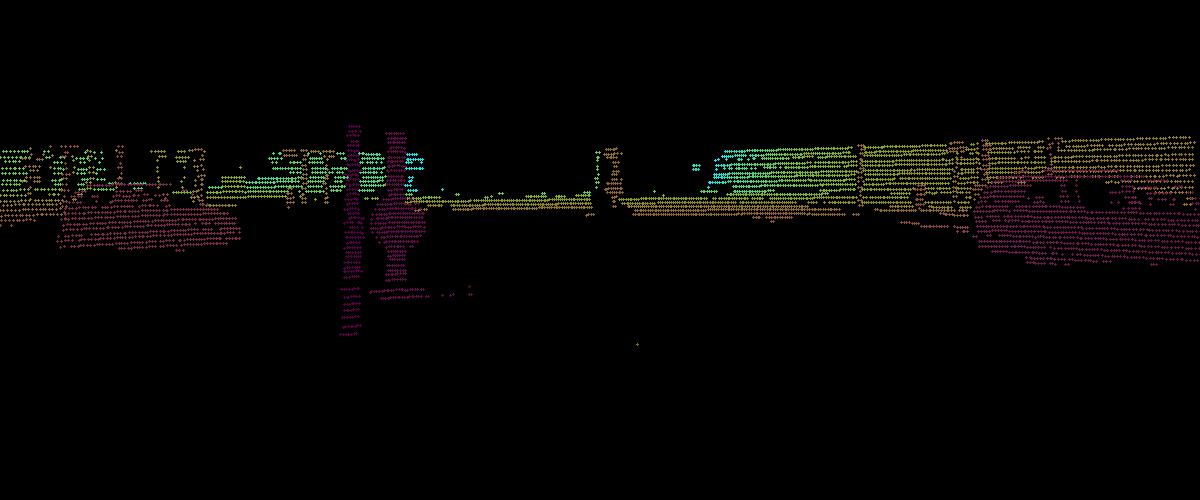
\includegraphics[width=\linewidth]{LidarImageTransformed.png}
  \caption{LiDAR transformed Data}
  \label{LiDAR transformed Data}
\end{figure}

The bin data was hard to project on this reference, so I converted to a 2D image[Fig 14] with removing the plain with highest noise (road in the background) to capture all the items of importance and that are nearby, within a certain range.

\begin{figure}[htbp]
  \centering
  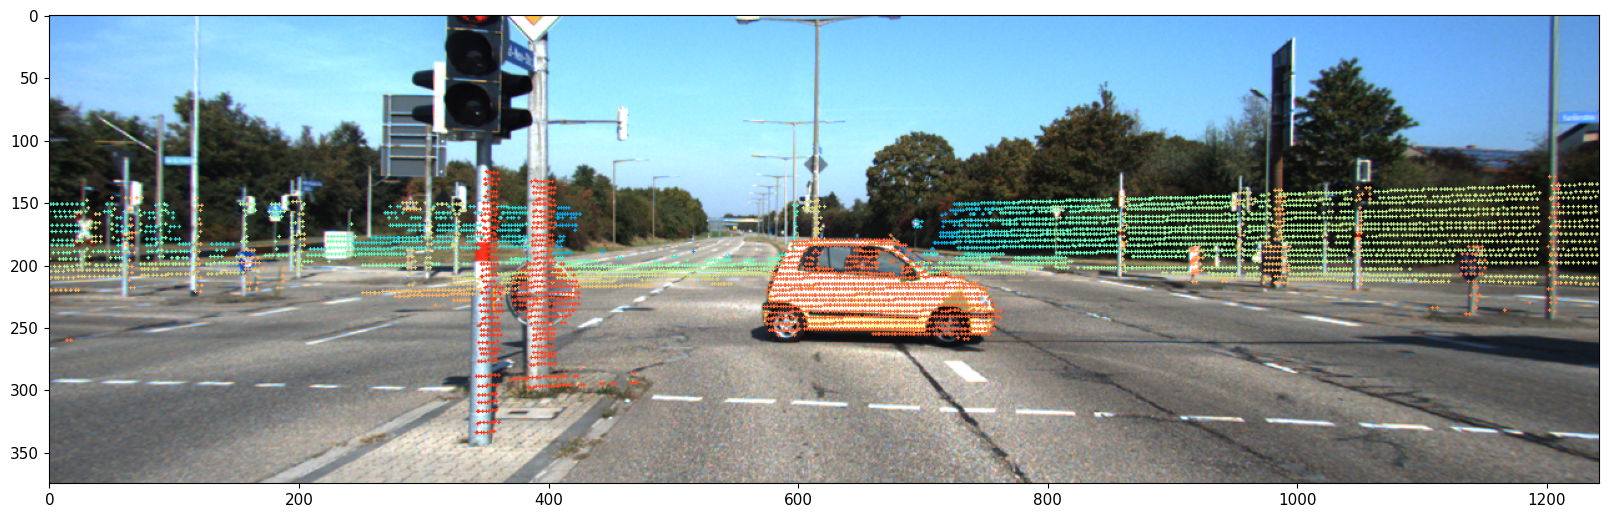
\includegraphics[width=\linewidth]{LidarOnTop.png}
  \caption{LiDAR on top of Camera}
  \label{LiDAR on top of Camera}
\end{figure}

\begin{figure}[htbp]
  \centering
  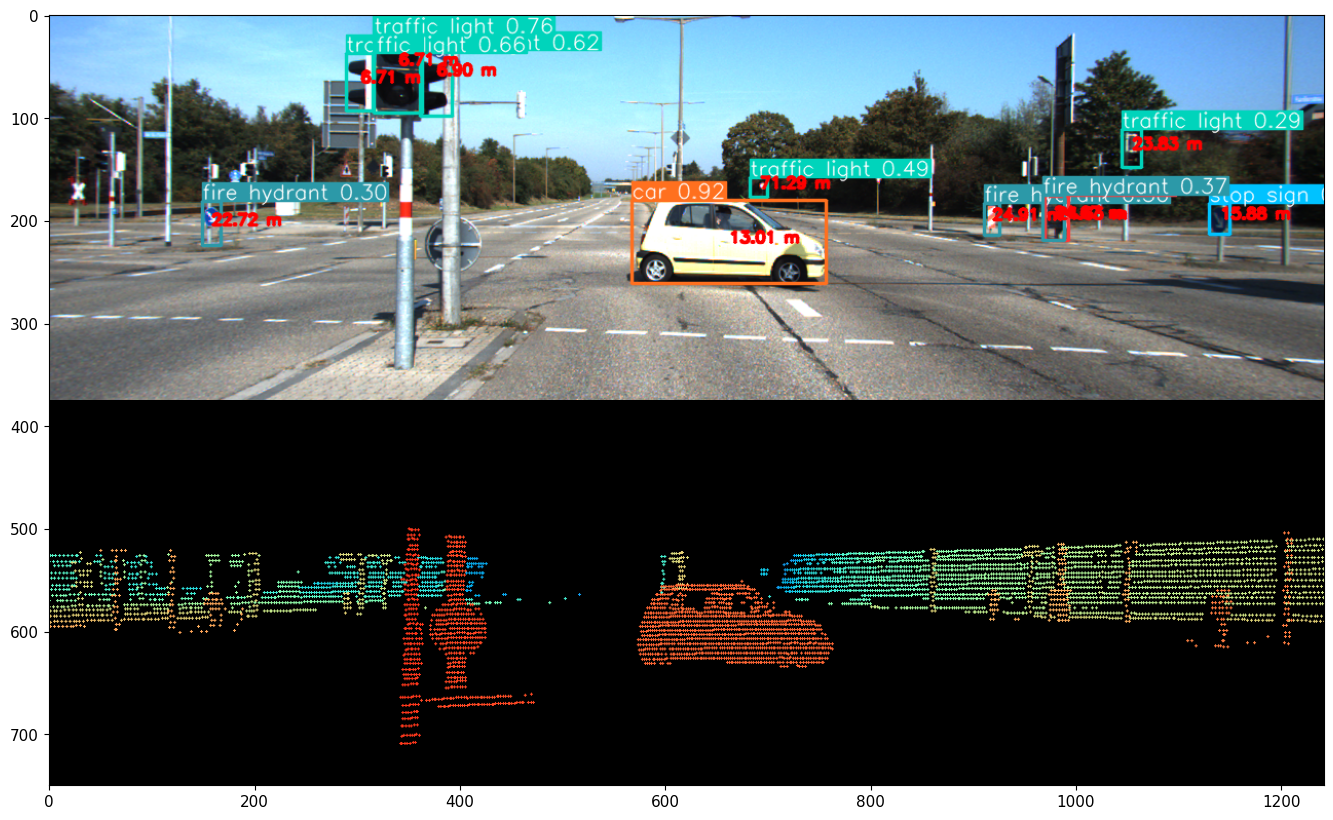
\includegraphics[width=\linewidth]{stacked.png}
  \caption{Comparision of data}
  \label{Comparision of data}
\end{figure}


\begin{figure}[htbp]
  \centering
  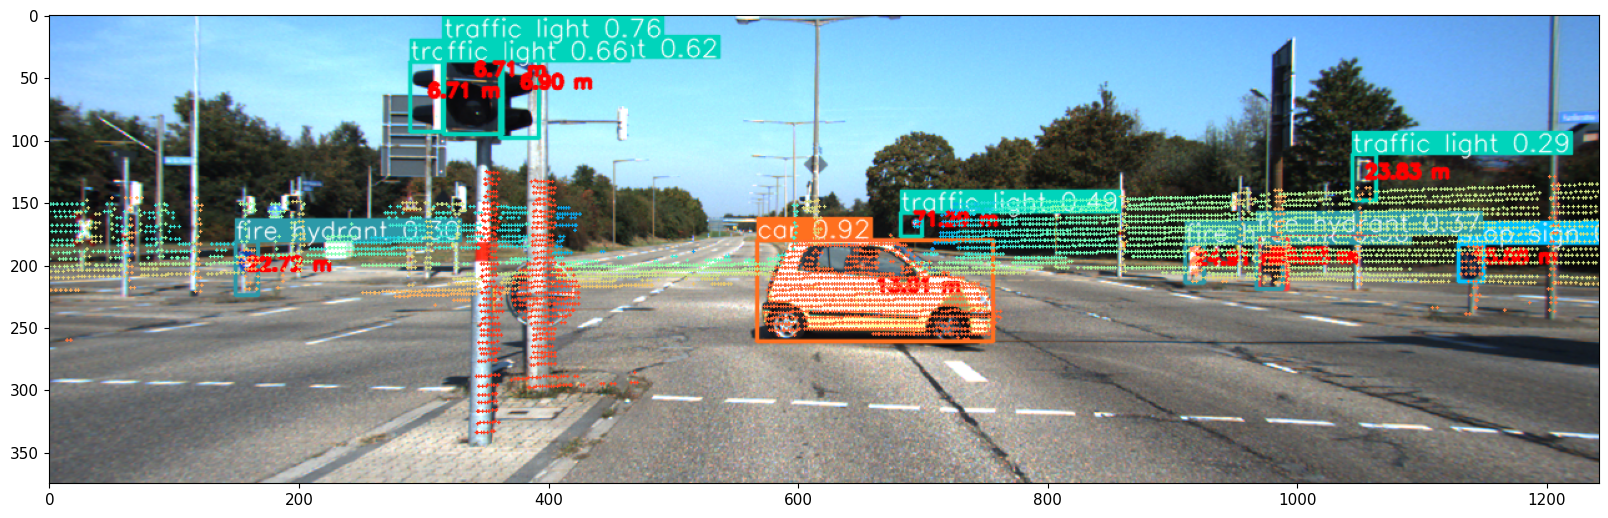
\includegraphics[width=\linewidth]{CameraLidarFinalFusion.png}
  \caption{Camera Lidar Final Fusion}
  \label{Camera Lidar Final Fusion}
\end{figure}


\section{CONCLUSIONS}

From this paper, I gained insights on how KITTI dataset functions. I was able to explore ROS integration along with C++/Python libraries. I understand the basics of computer vision, the importance of homegenous matrices. I understood the forward conversion of Velodyne data to Camera data, and also explored the backward transformation for Camera to LiDAR.

By the implementation of paper \cite{KITTI}, \cite{CameraCalibration} and \cite{CoordinateTransforms}, I got some background on Sensor Fusion between Camera and LiDAR on the KITTI dataset. Although it is challenging to read Velodyne data byitself, we can reduce the load and giving it only certain boxes that it is supposed to look into to get the depth or distance to that object.



\addtolength{\textheight}{-12cm}   % This command serves to balance the column lengths
                                  % on the last page of the document manually. It shortens
                                  % the textheight of the last page by a suitable amount.
                                  % This command does not take effect until the next page
                                  % so it should come on the page before the last. Make
                                  % sure that you do not shorten the textheight too much.

%%%%%%%%%%%%%%%%%%%%%%%%%%%%%%%%%%%%%%%%%%%%%%%%%%%%%%%%%%%%%%%%%%%%%%%%%%%%%%%%



%%%%%%%%%%%%%%%%%%%%%%%%%%%%%%%%%%%%%%%%%%%%%%%%%%%%%%%%%%%%%%%%%%%%%%%%%%%%%%%%



%%%%%%%%%%%%%%%%%%%%%%%%%%%%%%%%%%%%%%%%%%%%%%%%%%%%%%%%%%%%%%%%%%%%%%%%%%%%%%%%



%%%%%%%%%%%%%%%%%%%%%%%%%%%%%%%%%%%%%%%%%%%%%%%%%%%%%%%%%%%%%%%%%%%%%%%%%%%%%%%%


\begin{thebibliography}{99}

\bibitem{NVIDIA} NVIDIA, "How Does a Self-Driving Car See?," NVIDIA Blog, 2023. [Online]. Available: https://blogs.nvidia.com/blog/how-does-a-self-driving-car-see/. [Accessed: Dec. 05, 2023].

\bibitem{KITTI} A. Geiger, P. Lenz, C. Stiller, and R. Urtasun, "Vision meets Robotics: The KITTI Dataset," in International Journal of Robotics Research (IJRR), 2013.

\bibitem{KITTIWebsite} KITTI Website link; "https://www.cvlibs.net/datasets/kitti/"

\bibitem{PointPainting3DObject} Sourabh Vora, Alex H. Lang, Bassam Helou, Oscar Beijbom. "PointPainting: Sequential Fusion for 3D Object Detection," 2019.

\bibitem{CameraCalibration} A. Geiger, F. Moosmann, O. Car, and B. Schuster, "A toolbox for automatic calibration of range and camera sensors using a single shot," in Proceedings of the International Conference on Robotics and Automation (ICRA), 2012.

\bibitem{CoordinateTransforms} Coordinate Transforms for Sensor Fusion; "https://medium.com/@itberrios6/coordinate-transforms-for-sensor-fusion-40de05a6acf4"


\end{thebibliography}



\end{document}
 